% -*- coding: iso-2022-jp -*-
%%%%%%%%
% To control hyperref on command line,
% you can select one of (1),(2a),(2b),(3).
%   (1) do not treat hyperref
%   $ uplatex bkmk-jis.tex
%   (2a) hyperref + dvipdfmx (with CMap conversion)
%   $ uplatex "\def\withhyperref{dvipdfmx}\input" bkmk-jis.tex
%   (2b) hyperref + dvipdfmx + "convbkmk.rb -o"/out2uni (w/o CMap conversion)
%   $ uplatex "\def\withhyperref{dvipdfmx}\def\nocmap{true}\input" bkmk-jis.tex
%   (3) hyperref + dvips + convbkmk.rb + distiller/ps2pdf
%   $ uplatex "\def\withhyperref{dvips}\input" bkmk-jis.tex
%%%%%%

\newif\ifuptexmode\uptexmodefalse
\ifnum\jis"2121="3000

 %% for upLaTeX
 \def\pLaTeXorupLaTeX{upLaTeX}
 \uptexmodetrue
 \def\innerencoding{UPTEX}
 \def\cmap{UTF8-UTF16}

\else

 %% for pLaTeX
 \def\pLaTeXorupLaTeX{pLaTeX}
 \uptexmodefalse

 \ifnum\jis"2121="A1A1
  \def\innerencoding{EUC}
  \def\cmap{EUC-UCS2}
 \fi
 \ifnum\jis"2121="8140
  \def\innerencoding{SJIS}
  \def\cmap{90ms-RKSJ-UCS2}
 \fi

\fi

\makeatletter

\def\@opt@{multi}
\def\@default{default}
\def\@jarticle{jarticle}
\def\@tarticle{tarticle}
\def\@ujarticle{ujarticle}

\ifx\option\@undefined
 \def\option{default}
\fi

\ifx\class\@undefined
 \ifuptexmode
  \def\class{ujarticle}
 \else
  \def\class{jarticle}
 \fi
\fi
\ifuptexmode
 \edef\@opt@{uplatex,\@opt@}
\fi
\ifx\class\@jarticle
  \documentclass[a4paper,titlepage]{\class}
\else
 \ifx\class\@ujarticle
  \documentclass[a4paper,titlepage]{\class}
 \else
  \documentclass[a4paper,titlepage,landscape]{\class}
 \fi
\fi

\usepackage{graphicx}
\usepackage{textcomp}
\usepackage[\@opt@]{otf}

\def\@dvipdfmx{dvipdfmx}
\def\@dvips{dvips}

\ifx\withhyperref\@undefined
 \def\withhyperref{undefined}
 \def\texorpdfstring{%
   \expandafter\@firstoftwo
 }
\else
 \ifx\withhyperref\@dvipdfmx
  \def\@hyperrefkeyval{dvipdfm}
  \usepackage{atbegshi}
  \ifx\nocmap\@undefined
   \AtBeginShipoutFirst{\special{pdf:tounicode \cmap}}
  \else
   \def\cmap{---}
  \fi
 \fi
 \ifx\withhyperref\@dvips
  \def\@hyperrefkeyval{dvips}
 \fi

\ifx\nocmap\@undefined
 \usepackage[\@hyperrefkeyval,%
 bookmarks=true,%
 bookmarksnumbered=true,%
 bookmarkstype=toc,%
 %pdfstartview={FitBH -32768},%
 pdftitle={$B$$$m$$$m3N$+$a$F$_$k(B},%
 pdfsubject={hyperref$BJT(B},%
 pdfauthor={$BL>L5(B $B8"J<1R(B},%
 pdfkeywords={TeX; dvips; dvipdfmx; bookmark; hyperref; $B$7$*$j(B; pdf}%
 ]{hyperref}
\else
 \input bkmk-docinfo.out
 \usepackage[dvipdfm,%
 bookmarks=true,%
 bookmarksnumbered=true,%
 bookmarkstype=toc,%
 %pdfstartview={FitBH -32768},%
 pdftitle=\PDFTITLE,%
 pdfsubject=\PDFSUBJECT,%
 pdfauthor=\PDFAUTHOR,%
 pdfkeywords=\PDFKEYWORDS%
 ]{hyperref}
\fi

\fi

\makeatother

\title{$B$$$m$$$m3N$+$a$F$_$k(B}

\author{$BL>L5(B $B8"J<1R(B}

\oddsidemargin0mm
\evensidemargin0mm
\topmargin-15mm
\textwidth162mm
\textheight245mm

\edef\bs{$\backslash$\kern0em}

\begin{document}
\maketitle
\section{section title by ASCII}
test test.

hyperref with: \withhyperref
\makeatletter
\ifx\withhyperref\@dvipdfmx
 ~~CMap:\cmap
\fi
\makeatother
\typeout{### hyperref with: \withhyperref}

pLaTeX or upLaTeX: \pLaTeXorupLaTeX
\typeout{### pLaTeX or upLaTeX: \pLaTeXorupLaTeX}

inner encoding: \innerencoding
\typeout{### inner encoding: \innerencoding}

\begin{figure}
 \begin{center}
  \scalebox{0.2}{\includegraphics{box-jis.eps}}
  \caption{JIS$B$GId9f2=$5$l$?(BEPS$B%U%!%$%k(B}
  \label{fig:box-jis}
 \end{center}
\end{figure}
%\begin{figure}
% \begin{center}
%  \scalebox{0.2}{\includegraphics{box-sjis.eps}}
%  \caption{Shift\_JIS$B$GId9f2=$5$l$?(BEPS$B%U%!%$%k(B}
%  \label{fig:box-sjis}
% \end{center}
%\end{figure}
%\begin{figure}
% \begin{center}
%  \scalebox{0.2}{\includegraphics{box-euc.eps}}
%  \caption{EUC-JP$B$GId9f2=$5$l$?(BEPS$B%U%!%$%k(B}
%  \label{fig:box-euc}
% \end{center}
%\end{figure}
%\begin{figure}
% \begin{center}
%  \scalebox{0.2}{\includegraphics{box-utf8.eps}}
%  \caption{UTF-8$B$GId9f2=$5$l$?(BEPS$B%U%!%$%k(B}
%  \label{fig:box-utf8}
% \end{center}
%\end{figure}
\section{$B&A&B&C(B}
test test.

\section{$B'Q'R'S(B}
test test.

\section{$B%;%/%7%g%s(B}
test test.
\subsection{$B%5%V%;%/%7%g%s(B($B3g8L(B)}
test test.

\makeatletter
\ifx\withhyperref\@undefined
\else

\section{Escape sequences \texorpdfstring{\textbullet\textdagger\textdaggerdbl\ldots---\textflorin--\textperthousand\texttrademark\texteuro}%
{\200\201\202\203\204\206\205\213\222\240}$B$J$I(B}
\textbullet\textdagger\textdaggerdbl\ldots---\textflorin--\textperthousand\texttrademark\texteuro $B$J$I(B

\section{$B8+=P$7$K(B\texorpdfstring{\bs}{\134}UTF, \texorpdfstring{\bs}{\134}UTFC, \texorpdfstring{\bs}{\134}UTFM$B$J$I(B}
\subsection{$BF|K\!'(B\UTF{9aa8}\UTF{6D77} $B4JBN;z!'(B\UTFC{9aa8}\UTFC{6D77} $BHKqs;z!'(B\UTFT{9AA8}\UTFT{6d77} $BD+A/!'(B\UTFK{9AA8}\UTFK{6d77}}
$BF|K\!'(B\UTF{9aa8}\UTF{6D77} $B4JBN;z!'(B\UTFC{9aa8}\UTFC{6D77} $BHKqs;z!'(B\UTFT{9AA8}\UTFT{6d77} $BD+A/!'(B\UTFK{9AA8}\UTFK{6d77}

\subsection{$B%O%s%0%k!'(B\UTFK{c548}\UTFK{b155}\UTFK{d558}\UTFK{C138}\UTFK{C694}}
$B%O%s%0%k!'(B\UTFK{c548}\UTFK{b155}\UTFK{d558}\UTFK{C138}\UTFK{C694}

\subsection{$BF|K\!'(B\UTF{20509}\UTF{241FE}$B!!4JBN;z!'(B\UTFC{20509}\UTFC{241FE}  $BB?8@8l!'(B\UTFM{20509}\UTFM{241FE}}
$BF|K\!'(B\UTF{20509}\UTF{241FE}$B!!4JBN;z!'(B\UTFC{20509}\UTFC{241FE}  $BB?8@8l!'(B\UTFM{20509}\UTFM{241FE}

\subsection{$BF|K\!'(B\UTF{20509}\UTF{241FE}$B!!4JBN;z!'(B\UTFC{20509}\UTFC{241FE}  $BB?8@8l!'(B\UTFM{20509}\UTFM{241FE}}
$BF|K\!'(B\UTF{20509}\UTF{241FE}$B!!4JBN;z!'(B\UTFC{20509}\UTFC{241FE}  $BB?8@8l!'(B\UTFM{20509}\UTFM{241FE}

\subsection{$BF|K\!'(B\UTF{20b9f}\UTF{26402}$B!!HKqs;z!'(B\UTFT{20b9f}\UTFT{26402}  $BB?8@8l!'(B\UTFM{20b9f}\UTFM{26402}}
$BF|K\!'(B\UTF{20b9f}\UTF{26402}$B!!HKqs;z!'(B\UTFT{20b9f}\UTFT{26402}  $BB?8@8l!'(B\UTFM{20b9f}\UTFM{26402}

\subsection{$B4JBN;z!'(B\UTFC{20087}\UTFC{200cc}$B!!HKqs;z!'(B\UTFT{20087}\UTFT{200cc}  $BB?8@8l!'(B\UTFM{20087}\UTFM{200cc}}
$B4JBN;z!'(B\UTFC{20087}\UTFC{200cc}$B!!HKqs;z!'(B\UTFT{20087}\UTFT{200cc}  $BB?8@8l!'(B\UTFM{20087}\UTFM{200cc}
\fi
\makeatother

\end{document}
